% !TEX program = pdflatex
% !TEX options = -synctex=1 -interaction=nonstopmode -file-line-error "%DOC%"
% 固体物理第九次作业
\documentclass[UTF8,10pt,a4paper]{article}
\usepackage{ctex}
% \catcode`\。=\active
% \newcommand{。}{.}
\newcommand{\CourseName}{固体物理}
\newcommand{\CourseCode}{PHYS1502}
\newcommand{\Semester}{2019-2020学年第二学期}
\newcommand{\ProjectName}{第九次作业}
\newcommand{\DueTimeType}{截止时间}
\newcommand{\DueTime}{2020. 5. 8(周五)17:00}
\newcommand{\StudentName}{陈稼霖}
\newcommand{\StudentID}{45875852}
\usepackage[vmargin=1in,hmargin=.5in]{geometry}
\usepackage{fancyhdr}
\usepackage{lastpage}
\usepackage{calc}
\pagestyle{fancy}
\fancyhf{}
\fancyhead[L]{\CourseName}
\fancyhead[C]{\ProjectName}
\fancyhead[R]{\StudentName}
\fancyfoot[R]{\thepage\ / \pageref{LastPage}}
\setlength\headheight{12pt}
\fancypagestyle{FirstPageStyle}{
    \fancyhf{}
    \fancyhead[L]{\CourseName\\
        \CourseCode\\
        \Semester}
    \fancyhead[C]{{\Huge\bfseries\ProjectName}\\
        \DueTimeType\ : \DueTime}
    \fancyhead[R]{姓名 : \makebox[\widthof{\StudentID}][s]{\StudentName}\\
        学号 : \StudentID\\
        成绩 : \underline{\makebox[\widthof{\StudentID}]{}}}
    \fancyfoot[R]{\thepage\ / \pageref{LastPage}}
    \setlength\headheight{36pt}
}
\usepackage{amsmath,amssymb,amsthm,bm}
\allowdisplaybreaks[4]
\newtheoremstyle{Problem}
{}
{}
{}
{}
{\bfseries}
{.}
{ }
{第\thmnumber{ #2}\thmname{ #1}\thmnote{ (#3)} 得分: \underline{\qquad\qquad}}
\theoremstyle{Problem}
\newtheorem{prob}{题}
\newtheoremstyle{Solution}
{}
{}
{}
{}
{\bfseries}
{:}
{ }
{\thmname{#1}}
\makeatletter
\def\@endtheorem{\qed\endtrivlist\@endpefalse}
\makeatother
\theoremstyle{Solution}
\newtheorem*{sol}{解}
\providecommand{\abs}[1]{\left\lvert#1\right\rvert}
\usepackage{graphicx}
\begin{document}
\thispagestyle{FirstPageStyle}
\begin{prob}[(14.1) Reciprocal Lattice and X-ray Scattering]
    Consider the lattice described in Exercise 13.5 (a two-dimensional rectangular crystal having a unit cell with side $a_1=0.468$ nm and $a_2=0.342$ nm). A collimated beam of monochromatic X-ray with wavelength $0.166$ nm is used to examine the crystal.
    \begin{enumerate}
        \item[(a)] Draw to scale a diagram of the reciprocal lattice.
        \item[(b)] Calculate the magnitude of the wavevectors $\bm{k}$ and $\bm{k}'$ of the incident and reflected X-ray beams, and hence construct on your drawing the "scattering triangle" corresponding to the Laue condition $\Delta\bm{k}=\bm{G}$ for diffraction from the $(210)$ planes (the scattering triangle includes $\bm{k},\bm{k}'$ and $\Delta\bm{k}$.)
    \end{enumerate}
\end{prob}
\begin{sol}
    \begin{enumerate}
        \item[(a)] 二维矩形晶体的倒格子的基矢为
        \begin{align}
            \bm{b}_1=&\frac{2\pi\bm{a}_2\times\hat{z}}{\hat{z}\cdot(\bm{a}_1\times\bm{a}_2)}=\frac{2\pi\hat{a}_1}{\abs{\bm{a}_1}},\\
            \bm{b}_2=&\frac{2\pi\hat{z}\times\bm{a}_1}{\hat{z}\cdot(\bm{a}_1\times\bm{a}_2)}=\frac{2\pi\hat{a}_2}{\abs{\bm{a}_2}}.
        \end{align}
        因此倒格子的基矢$\bm{b}_1$的长度为$\frac{2\pi}{\abs{\bm{a}_1}}=13.4nm^{-1}$,$\bm{b}_2$的长度为$\frac{2\pi}{\abs{\bm{a}_2}}=18.4nm^{-1}$,两者相互垂直. 倒格子如图\ref{1-RL}.
        \item[(b)] 入射和出射的X射线的波矢长度均为
        \begin{align}
            \abs{\bm{k}}=\abs{\bm{k}'}=\frac{2\pi}{\lambda}=37.9\text{nm}^{-1}.
        \end{align}
        由于与$(210)$晶面发生散射,根据劳厄条件,入射波矢和出射波矢之差即为由倒格子中原点$(000)$指向点$(210)$的矢量,分别以原点$(000)$和点$(210)$为圆心,以$37.9\text{nm}^{-1}$为半径画圆,两圆交点指向两圆心的矢量即为入射和出射波矢,这三个矢量所围三角形即为满足劳厄条件的散射三角形,如图\ref{1-RL}.
        \begin{figure}[h]
            \centering
            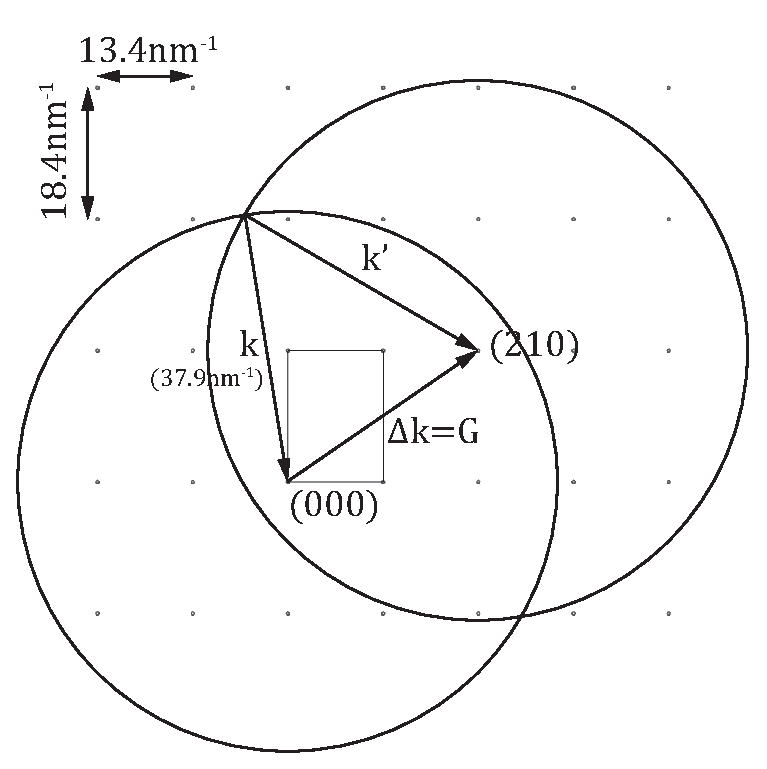
\includegraphics[width=.4\textwidth]{1.eps}
            \caption{倒格子及满足劳厄条件的散射三角形.}
            \label{1-RL}
        \end{figure}
    \end{enumerate}
\end{sol}

\begin{prob}[(14.2) $\ddagger$X-ray scattering II]
    BaTiO$_3$ has a primitive cubic lattice and a basis with atoms having fractional coordinates
    \begin{align*}
        \text{Ba}\quad&[0,0,0]\\
        \text{Ti}\quad&[\frac{1}{2},\frac{1}{2},\frac{1}{2}]\\
        \text{O}\quad&[\frac{1}{2},\frac{1}{2},0],\quad[\frac{1}{2},0,\frac{1}{2}]\quad[0,\frac{1}{2},\frac{1}{2}]
    \end{align*}
    \begin{itemize}
        \item[$\triangleright$] Sketch the unit cell.
        \item[$\triangleright$] Show that the X-ray structure factor for the $(00l)$ Bragg reflection is given by
        \[
            S_{(hkl)}=f_{Ba}+(-1)^lf_{Ti}+\left[1+2(-1)^l\right]f_O
        \]
        where $f_{Ba}$ is the atomic form factor for Ba, etc.
        \item[$\triangleright$] Calculate the ratio $I_{(002)}/I_{(001)}$, where $I_{(hkl)}$ is the intensity of the X-ray diffraction from the $(hkl)$ planes. You may assume that the atomic form factor is proportional to atomic number ($Z$), and neglect its dependence on the scattering vector. ($Z_{Ba}=56$, $Z_{Ti}=22$, $Z_O=8$.)
    \end{itemize}
\end{prob}
\begin{sol}
    \begin{itemize}
        \item[$\triangleright$] BaTiO$_3$的原胞如图\ref{2-UC}.
        \begin{figure}[h]
            \centering
            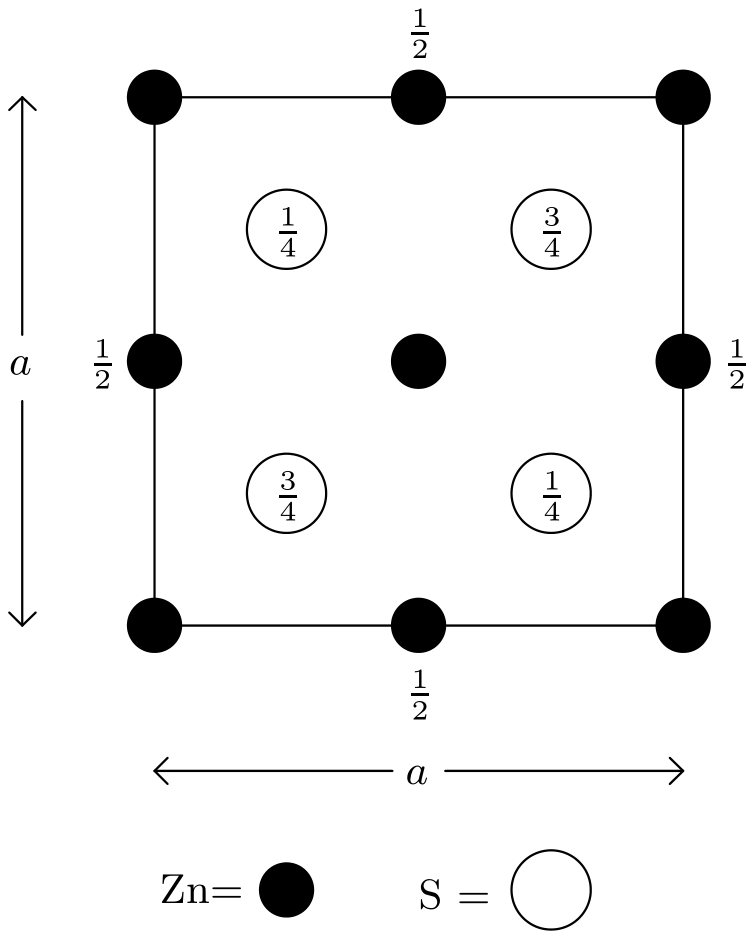
\includegraphics[width=.6\textwidth]{2.eps}
            \caption{BaTiO$_3$的原胞,其中绿色小球代表Ba原子,蓝色小球代表Ti原子,红色小球代表O原子.}
            \label{2-UC}
        \end{figure}
        \item[$\triangleright$] 对$(00l)$布拉衍射,结构因子为
        \begin{align}
            \nonumber S_{(001)}=&e^{2\pi i(0,0,l)\cdot(0,0,0)}f_{Ba}+e^{2\pi i(0,0,l)\cdot(\frac{1}{2},\frac{1}{2},\frac{1}{2})}f_{Ti}+[e^{2\pi i(0,0,l)\cdot(\frac{1}{2},\frac{1}{2},0)}+e^{2\pi i(0,0,l)\cdot(\frac{1}{2},0,\frac{1}{2})}+e^{2\pi i(0,0,l)\cdot(0,\frac{1}{2},\frac{1}{2})}]f_O\\
            =&f_{Ba}+(-1)^lf_{Ti}+[1+2(-1)^l]f_O.
        \end{align}
        \item[$\triangleright$] 假设原子的形状因子仅与其原子序数成正比,因衍射强度正比结构因子的平方,$I_{hkl}\propto S^2$,故$(002)$平面与$(001)$晶面衍射的光强之比为
        \begin{align}
            \frac{I_{002}}{I_{001}}=\frac{S_{(002)}^2}{S_{(001)}^2}=\frac{(f_{Ba}+f_{Ti}-f_O)^2}{(f_{Ba}-f_{Ti}+3f_O)^2}=\frac{(56+22+3\times 8)^2}{(56-22-8)^2}=15.4.
        \end{align}
    \end{itemize}
\end{sol}

\begin{prob}[(14.3) $\ddagger$X-ray scattering and Systematic Absence]
    \begin{enumerate}
        \item[(a)] Explain what is meant by "Lattice Constant" for a cubic crystal structure.
        \item[(b)] Explain why X-ray diffraction may be observed in first order from the $(110)$ planes of a crystal with a body-centered cubic lattice, but not from the $(110)$ planes of a crystal with a face-centered cubic lattice.
        \begin{itemize}
            \item[$\triangleright$] Derive the general selection rules for which planes are observed in bcc and fcc lattice.
        \end{itemize}
        \item[(c)] Show that these selection rules hold independent of what atoms are in the primitive unit cell, so long as the lattice is bcc or fcc respectively.
        \item[(d)] A collimated beam of monochromatic X-rays of wavelength $0.162$ nm is incident upon a powdered sample of the cubic metal palladium. Peaks in the scattered X-ray pattern are observed at angles of $42.3^{\circ}$, $49.2^{\circ}$, $72.2^{\circ}$, $87.4^{\circ}$, and $92.3^{\circ}$ from the direction of the incident beam.
        \begin{itemize}
            \item[$\triangleright$] Identify the lattice type.
            \item[$\triangleright$] Calculate the lattice constant and the nearest-neighbor distance.
            \item[$\triangleright$] If you assume there is only a single atom in the basis does this distance agree with the known data that the density of palladium is $12023\text{ kg m}^{-3}$? (Atomic mass of palladium $=106.4$.)
        \end{itemize}
        \item[(e)] How could you improve the precision with which the lattice constant is determined. (For one suggestion, see Exercise 14.10.)
    \end{enumerate}
\end{prob}
\begin{sol}
    \begin{enumerate}
        \item[(a)] 对于立方晶系,晶格常数指的是一个格点到与之最近的另一个格点的距离.
        \item[(b)] bcc格子的结构因子为
        \begin{align}
            \label{3-bcc-S}
            \nonumber S_{(hkl)}^{bcc}=&e^{2\pi i(h,k,l)\cdot(0,0,0)}f_{\text{lattice point}}+e^{2\pi i(h,k,l)\cdot(\frac{1}{2},\frac{1}{2},\frac{1}{2})}f_{\text{lattice point}}\\
            =&[1+(-1)^{h+k+l}]f_{\text{lattice point}},
        \end{align}
        其中$f_{\text{lattice point}}$是结构因子中对一个格点(结构基元)中的所有原子的形状因子(并且考虑这些原子间的相对位置,带有传播相因子)的求和的部分,见式\ref{3-fLP}.\\
        fcc格子的结构因子为
        \begin{align}
            \label{3-fcc-S}
            \nonumber S_{(hkl)}^{fcc}=&e^{2\pi i(h,k,l)\cdot(0,0,0)}f_{\text{lattice point}}+e^{2\pi i(h,k,l)\cdot(\frac{1}{2},\frac{1}{2},0)}f_{\text{lattice point}}+e^{2\pi i(h,k,l)\cdot(\frac{1}{2},0,\frac{1}{2})}f_{\text{lattice point}}\\
            \nonumber&+e^{2\pi i(h,k,l)\cdot(0,\frac{1}{2},\frac{1}{2})}f_{\text{lattice point}}\\
            =&[1+(-1)^{h+k}+(-1)^{h+l}+(-1)^{k+l}]f_{\text{lattice point}}.
        \end{align}
        对于来自$(110)$晶面的衍射,对于bcc格子,结构因子为
        \begin{align}
            S_{(110)}^{bcc}=2f_{\text{lattice point}},
        \end{align}
        故可以观测到散射信号.\\
        对于fcc格子,结构因子为
        \begin{align}
            S_{(110)}^{fcc}=0,
        \end{align}
        故无法观测到衍射信号.
        \begin{itemize}
            \item[$\triangleright$] 一般性的消光规律:对于bcc格子,根据式\ref{3-bcc-S},当$(h+k+l)$为偶数时,可以观察到衍射信号;当$(h+k+l)$为奇数时,无法观察到衍射信号.\\
            对于fcc格子,根据式\ref{3-fcc-S},仅当$h,k,l$这三个数全为奇数或全为偶数时,才可以观测到衍射信号;在其他情况下,无法观测到衍射信号.
        \end{itemize}
        \item[(c)] 由于式\ref{3-bcc-S}和式\ref{3-fcc-S}中的
        \begin{align}
            \label{3-fLP}
            f_{\text{lattice point}}=\sum_jf_je^{i\bm{k}_{(hkl)}\cdot\bm{r}_j}
        \end{align}
        (上面的求和是对于一个结构基元中的所有原子进行,其中$f_j$和$\bm{r}_j$分别为结构基元中第$j$个原子的形状因子和位置)\\
        仅为一个系数,对于式子的是否等于零没有影响,故上面得到的这些消光规律不受原胞中具体原子种类的影响.
        \item[(d)] 用布拉格公式
        \begin{align}
            d=\frac{\lambda}{2\sin\theta}
        \end{align}
        计算各个角度对应的晶面间距,从最大晶面间距与各晶面间距的商的平方,我们可以推出各个晶面的Miller指数,结果如表\ref{3-T}.
        \begin{table}[h]
            \centering
            \caption{}
            \label{3-T}
            \begin{tabular}{cccc}
            \hline
            $2\theta$ & 晶面间距$d=\frac{\lambda}{2\sin\theta}$ & 最大晶面间距与当前晶面间距的商的平方$\left(\frac{d_{\max}}{d}\right)^2$ & Miller指数(无顺序) \\ \hline
            $42.3^{\circ}$ & $0.224$nm & $1=\frac{1^2+1^2+1^2}{3}$ & $(1,1,1)$ \\
            $49.2^{\circ}$ & $0.195$nm & $1.33=\frac{1^2+1^2+2^2}{3}$ & $(0,0,2)$ \\
            $72.2^{\circ}$ & $0.137$nm & $2.67=\frac{2^2+2^2+2^2}{3}$ & $(2,2,2)$ \\
            $87.4^{\circ}$ & $0.117$nm & $3.67=\frac{1^2+1^2+3^2}{3}$ & $(1,1,3)$ \\
            $92.3^{\circ}$ & $0.112$nm & $4.00=\frac{2^2+2^2+2^2}{3}$ & $(2,2,2)$ \\ \hline
            \end{tabular}
        \end{table}
        \begin{itemize}
            \item[$\triangleright$] 从表\ref{3-T}中可见,所有的衍射信号均对应着$h,k,l$这三个数要么全为偶数,要么全为奇数,根据上面得到的结论,晶格类型为fcc.
            \item[$\triangleright$] 晶格常数为
            \begin{align}
                a=d\sqrt{h^2+k^2+l^2}=0.112\text{nm}\times\sqrt{2^2+2^2+2^2}=0.389\text{nm}.
            \end{align}
            最近的两个原子间的距离为
            \begin{align}
                \frac{a}{\sqrt{2}}a=0.275\text{nm}.
            \end{align}
            \item[$\triangleright$] 若每个格点只含$1$个原子,则钯的密度为
            \begin{align}
                \rho=\frac{4\times\frac{106.4\times 10^{-3}}{6.02\times 10^{23}}\text{kg}}{(0.389\times 10^{-9}m)^3}=12010\text{kg m}^{-3}.
            \end{align}
            这一结果与已知的钯的密度$12023\text{kg m}^{-3}$符合得很好.
        \end{itemize}
        \item[(e)] 提高晶格常数测算精度的方法:
        \begin{itemize}
            \item 由于根据布拉格公式,$\frac{1}{d}\frac{\partial d}{\partial\theta}\approx\cot\theta$,对于角度$\theta$的给定误差,$\theta$越接近$\frac{\pi}{2}$,计算得到晶面间距的误差就越小,因此衍射实验尽可能用大的$\theta$;
            \item 提高X射线的强度以提高信噪比;
            \item 更好的聚焦以及更加精密的旋转晶体和测量角度的仪器以提高角度测量的精度;
            \item 更加精确地确定X射线的波长;
            \item 尽可能地控制样品温度稳定,以防止温度改变影响晶格常数.
        \end{itemize}
    \end{enumerate}
\end{sol}

\begin{prob}[(14.5) And More X-ray Scattering]
    A sample of aluminum powder is put in an Debye-Scherrer X-ray diffraction device. The incident X-ray radiation is from Cu-Ka X-ray transition (this just means that the wavelength is $\lambda=.154$ nm). The following scattering angles were observed:\\
    $19.48^{\circ}$ $22.64^{\circ}$ $33.00^{\circ}$ $39.68^{\circ}$ $41.83^{\circ}$ $50.35^{\circ}$ $57.05^{\circ}$\\
    Given also that the atomic weight of Al is $27$, and the density is $2.7\text{ g/cm}^3$, use this information to calculate Avagadro's number. How far off are you? What cause the error?
\end{prob}
\begin{sol}
    这一题干中并没有提到铝是立方晶系,但是如果没有这个条件的话,似乎很难单纯从衍射角度推迟晶格常数,因此我们查阅资料得知铝为fcc格子,下面只是用题干提供的实验数据来验证这一点. 用布拉格公式
    \begin{align}
        d=\frac{\lambda}{2\sin\theta}
    \end{align}
    计算各个角度对应的晶面间距,从最大晶面间距与各晶面间距的商的平方,我们可以推出各个晶面的Miller指数,结果如表\ref{4-T}.
    \begin{table}[h]
        \centering
        \caption{}
        \label{4-T}
        \begin{tabular}{cccc}
        \hline
        $\theta$ & 晶面间距$d=\frac{\lambda}{2\sin\theta}$ & 最大晶面间距与当前晶面间距的商的平方$\left(\frac{d_{\max}}{d}\right)^2$ & Miller指数(无顺序) \\ \hline
        $19.48^{\circ}$ & $0.231$nm & $1=\frac{1^2+1^2+1^2}{3}$ & $(1,1,1)$ \\
        $22.64^{\circ}$ & $0.200$nm & $1.33=\frac{1^2+1^2+2^2}{3}$ & $(1,1,2)$ \\
        $33.00^{\circ}$ & $0.141$nm & $2.67=\frac{2^2+2^2+2^2}{3}$ & $(2,2,2)$ \\
        $39.68^{\circ}$ & $0.121$nm & $3.67=\frac{1^2+1^2+3^2}{3}$ & $(1,2,3)$ \\
        $41.83^{\circ}$ & $0.115$nm & $4.00=\frac{2^2+2^2+2^2}{3}$ & $(2,2,2)$ \\
        $50.35^{\circ}$ & $0.100$nm & $5.33=\frac{0^2+0^2+4^2}{3}$ & $(0,0,4)$ \\
        $57.05^{\circ}$ & $0.0918$nm & $6.33=\frac{1^2+3^2+3^2}{3}$ & $(1,1,3)$ \\ \hline
        \end{tabular}
    \end{table}
    \\根据上一题得到的结论,铝的晶格类型属于fcc. 铝的晶格常数为
    \begin{align}
        a=d\sqrt{h^2+k^2+l^2}=0.0918\text{nm}\times\sqrt{1^2+3^2+3^2}=0.400\text{nm}.
    \end{align}
    若每个格点包含$1$个原子,则铝的密度可表为
    \begin{align}
        \rho=\frac{4\times\frac{27\times 10^{-3}\text{kg}\cdot\text{mol}^{-1}}{N_A}}{(0.400\times 10^{-9}\text{m})^3}=2.7\times 10^3\text{kg}/\text{m}^3.
    \end{align}
    解得阿伏伽德罗常数为
    \begin{align}
        N_A=6.25\times 10^{23}\text{mol}^{-1}.
    \end{align}
    所得结果与阿伏伽德罗常数的参考值相差$4\%$,误差来源
    \begin{itemize}
        \item 铝的原子量和密度的给定值的有效位数比较少;
        \item 给定的铝的密度对应的温度和进行X射线衍射实验的实验室温度不相等.
    \end{itemize}
\end{sol}

\begin{prob}[(14.9) From Factors]
    \begin{enumerate}
        \item[(a)] Assume that the scattering potential can be written as the sum over the contributions of the scattering from each of the atoms in the system. Write the positions of the atoms in terms of a lattice plus a basis so that
        \[
            V(\bm{x})=\sum_{\bm{R},\alpha}V_{\alpha}(\bm{x}-\bm{R}-\bm{y}_{\alpha})
        \]
        where $\bm{R}$ are lattice points, $\alpha$ indexed the particles in the basis and $\bm{y}_{\alpha}$ is the position of atom $\alpha$ in the basis. Now use the definition of the structure factor Eq. 14.5 and derive an expression of the form of Eq. 14.8 and hence derive expression 14.9 for the from factor. (Hint: Use the factor that an integral over all space can be decomposed into a sum over integrals of individual unit cells.)
        \item[(b)] Given the equation for the form factor you just derived (Eq. 14.9), assume the scattering potential from an atom is constant inside a radius $a$ and is zero outside that radius. Derive Eq. 14.10.
        \item[(c)$^*$] Use your knowledge of the wavefunction of an electron in a hydrogen atom to calculate the X-ray form factor of hydrogen.
    \end{enumerate}
\end{prob}
\begin{sol}
    \begin{enumerate}
        \item[(a)] 根据式(14.5),结构因子为
        \begin{align}
            S(\bm{G})=\int_{\text{unit cell}}d\bm{x}\,e^{i\bm{G}\cdot\bm{x}}V(\bm{x}).
        \end{align}
        代入
        \begin{align}
            V(\bm{x})=\sum_{\bm{R},\alpha}V(\bm{x}-\bm{R}-\bm{y}_{\alpha})
        \end{align}
        得
        \begin{align}
            \nonumber S=&\sum_{\bm{R}}\sum_{\alpha}\int_{\text{unit cell}}d\bm{x}\,e^{i\bm{G}\cdot\bm{x}}V(\bm{x}-\bm{R}-\bm{y}_{\alpha})\\
            \nonumber=&\sum_{\bm{R}}\sum_{\alpha}\int_{\text{unit cell}}d\bm{x}\,e^{i\bm{G}\cdot(\bm{x}-\bm{R}-\bm{y}_{\alpha})}e^{i\bm{G}\cdot(\bm{R}+\bm{y}_{\alpha})}V(\bm{x}-\bm{R}-\bm{y}_{\alpha})\\
            \nonumber&(\text{设}\bm{r}=\bm{x}-\bm{R}-\bm{y}_{\alpha})\\
            \nonumber=&\sum_{\bm{R}}\sum_{\alpha}e^{i\bm{G}\cdot(\bm{R}+\bm{y}_{\alpha})}\int_{\text{unit cell}}d\bm{x}\,e^{i\bm{G}\cdot\bm{r}}V_{\alpha}(\bm{r})\\
            \nonumber=&\sum_{\bm{R}}\sum_{\alpha}e^{i\bm{G}\cdot\bm{y}_{\alpha}}\int_{\text{unit cell}}d\bm{x}\,e^{i\bm{G}\cdot\bm{r}}V_{\alpha}(\bm{r})\\
            \nonumber=&\sum_{\alpha}e^{i\bm{G}\cdot\bm{y}_{\alpha}}\sum_{\bm{R}}\int_{\text{unit cell}}d\bm{x}\,e^{i\bm{G}\cdot\bm{r}}V_{\alpha}(\bm{r})\\
            \nonumber=&\sum_{\alpha}e^{i\bm{G}\cdot\bm{y}_{\alpha}}\int_{\text{all space}}d\bm{x}\,e^{i\bm{G}\cdot\bm{r}}V_{\alpha}(\bm{r})\\
            =&\sum_{\alpha}e^{i\bm{G}\cdot\bm{y}_{\alpha}}f_{\alpha}(\bm{G}),
        \end{align}
        其中形状因子
        \begin{align}
            f_{\alpha}(\bm{G})=\int_{\text{all space}}d\bm{r}\,V_{\alpha}(\bm{r})e^{i\bm{G}\cdot\bm{r}}.
        \end{align}
        \item[(b)] 假设
        \begin{align}
            V_{\alpha}(\bm{G})=\left\{\begin{array}{ll}
                V_0,&\abs{\bm{r}}\leq a,\\
                0,&\abs{\bm{r}}>a.
            \end{array}\right.
        \end{align}
        则形状因子
        \begin{align}
            \nonumber f_{\alpha}(\bm{G})=&\int_{\text{all space}}d\bm{r}\,V_{\alpha}(\bm{r})e^{i\bm{G}\cdot\bm{r}}\\
            \nonumber&(\text{其中$\theta$为$\bm{G}$和$\bm{r}$间的夹角})\\
            \nonumber=&2\pi V_0\int_0^ar^2\,dr\int_0^{\pi}\sin\theta\,d\theta\,e^{iGr\cos\theta}\\
            \nonumber=&2\pi V_0\int_0^ar^2\,dr\int_{-1}^1d(\cos\theta)\,e^{iGr\cos\theta}\\
            \nonumber=&2\pi V_0\int_0^ar^2\,dr\frac{2\sin(Gr)}{Gr}\\
            \nonumber=&\frac{4\pi V_0}{G^2}\left[\frac{\sin(Ga)}{G}-a\cos(Ga)\right]\\
            =&3\frac{4\pi}{3}V_0a^3\frac{\sin x-x\cos x}{x^3}.
        \end{align}
        其中$x=Gr$. 因为原子周围的电场强度大小正比核电荷数,$V_0\propto Z_{\alpha}$,故
        \begin{align}
            f_{\alpha}(\bm{G})\propto 3Z_{\alpha}\frac{\sin x-x\cos x}{x^3}.
        \end{align}
        \item[(c)] 基态氢原子的波函数为
        \begin{align}
            \psi(\bm{r})=\frac{1}{\sqrt{\pi a^3}}e^{-r/a}.
        \end{align}
        其中$a$为波尔半径. 散射势正比电子密度,设这一比值为$K$. 形状因子
        \begin{align}
            \nonumber f_{\alpha}(\bm{G})=&\int_{\text{all space}}d\bm{r}\,e^{i\bm{G}\cdot\bm{r}}K\abs{\psi(\bm{r})}^2\\
            \nonumber=&\frac{2K}{a^3}\int_0^{+\infty}r^2\,dr\int_0^{\pi}\sin\theta\,d\theta\,e^{iGr\cos\theta}e^{-2r/a}\\
            \nonumber=&\frac{2K}{a^3}\int_0^{+\infty}r^2\,dr\,\frac{2\sin(Gr)}{Gr}e^{-2r/a}\\
            \nonumber=&\frac{4\pi}{a^3G}\text{Im}\left[\int_0^{+\infty}re^{r(iG-2/a)}\,dr\right]\\
            \nonumber=&\frac{4K}{a^3G}\text{Im}\left[\frac{1}{4/a^2-G^2-4iG/a}\right]\\
            =&\frac{16K}{(G^2a^2+4)^2}.
        \end{align}
    \end{enumerate}
\end{sol}

\begin{prob}[(14.10)]
    Imagine you are trying to measure the lattice constant $a$ of some crystal using X-ray. Suppose a diffraction peak is observed at a scattering angle of $2\theta$. However, suppose that the value $\theta$ is measured only within some uncertainty $\delta\theta$. What is the fractional error $\delta a/a$ in the resulting measurement of the lattice constant? How might this error be reduced? Why could it not be reduced to zero?
\end{prob}
\begin{sol}
    若以$(100)$这样的晶面为反射面,可以根据布拉格公式
    \begin{align}
        a=\frac{\lambda}{2\sin\theta},
    \end{align}
    直接得到晶格常数,角度测量的不确定度$\delta\theta$造成的晶格常数的相对误差为
    \begin{gather}
        \frac{1}{d}\frac{\partial d}{\partial\theta}=\cot\theta\\
        \Longrightarrow\frac{\delta a}{a}=\cot\theta(\delta\theta).
    \end{gather}
    实验时使用尽可能接近$\frac{\pi}{2}$的$\theta$可以减少这样的误差. 但即使$\theta$无限接近$\frac{\pi}{2}$也无法完全消除误差,这是因为
    \begin{itemize}
        \item 上面计算得到的误差仅为一阶误差,更高阶的误差,如二阶相对误差$\frac{\delta a}{a}=\frac{1}{\sin^2\theta}(\delta\theta)^2$在$\theta=\frac{\pi}{2}$时仍不为零.
        \item 其他物理量和环境引起的误差,如入射X射线波长的误差、温度对晶格常数造成的误差(即使在绝对零度依然有统计物理的涨落效应影响晶格常数)等.
    \end{itemize}
\end{sol}

\begin{prob}[补充题]
    请计算用来做晶体衍射实验的x射线和中子的能量。x射线的波长选为0.166 nm,中子的波长选为0.123 nm。请利用本学期所学理论解释为什么选用这样的波长。
\end{prob}
\begin{sol}
    X射线的能量为
    \begin{align}
        E_X=\frac{hc}{\lambda}=\frac{6.63\times 10^{-34}\times 3\times 10^8}{0.166\times 10^{-9}}J=1.20\times 10^{-15}\text{J}=7488ev.
    \end{align}
    中子的能量为
    \begin{align}
        E_n=\frac{\left(\frac{h}{\lambda}\right)^2}{2m}=\frac{\left(\frac{6.63\times 10^{-34}}{0.123\times 10^{-9}}\right)^2}{2\times 1.67\times 10^{-27}}\text{J}=8.70\times 10^{-21}\text{J}=0.0544eV.
    \end{align}
    选择这样的波长的原因:根据劳厄公式
    \begin{align}
        \bm{k}'-\bm{k}=\bm{G}.
    \end{align}
    因为原子间距大约为$0.2$nm,故
    \begin{align}
        \abs{\bm{G}}\sim\frac{2\pi}{0.2\text{nm}}=31\text{nm}^{-1}
    \end{align}
    因为
    \begin{align}
        \abs{\bm{G}}=\abs{\bm{k}'-\bm{k}}\leq 2\abs{\bm{k}}=\frac{4\pi}{\lambda},
    \end{align}
    故满足劳厄公式的一个必要条件是:入射波的波长应当
    \begin{align}
        \lambda\leq 0.4\text{nm}.
    \end{align}
    故选择大约$0.1$nm波长的波入射是一个比较合理的值.
\end{sol}
\end{document}